\begin{frame}
	\frametitle{Models of varying complexity}
	
	\centering
	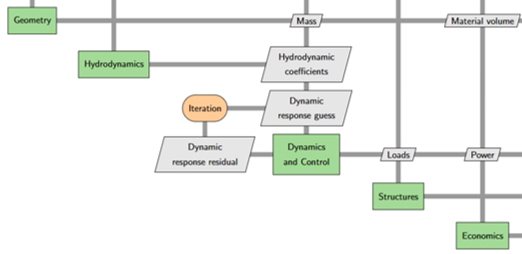
\includegraphics[width=0.9\linewidth]{figs/img0008.png}
	\begin{itemize}
		\item Algebraic
		      
		\item Linear PDE
		      
		\item Nonlinear ODE
		      
		\item Linear PDE
		      
		\item Algebraic
	\end{itemize}
	
\end{frame}


\begin{frame}
	\frametitle{Methods for Solving a PDE}
	\begin{itemize}
		\item Chosen methods
		\item Semi-analytical: dynamics,  hydrodynamics
		\item Analytical: structures
		\item Steps for each model
		\item Development
		\item Synthesis
		\item Validation
		\item Benchmarking
		      
		\item Accuracy
		      
		\item Compute time
		      
		\item Algebraic/Lumped
		      
		\item Numerical Linear
		      
		\item Numerical Nonlinear
		      
		\item (Semi-) Analytical
	\end{itemize}
	
\end{frame}


\begin{frame}
	\frametitle{Hydrodynamics: Matched Eigenfunction Expansion Method}
	\begin{itemize}
		\item Open-source Python toolbox: OpenFLASH
	\end{itemize}
	\begin{tabular}{|l|l|l|} \hline
		Geometry        & Mathematical development     & Open-source implementation    \\ \hline
		Simple cylinder & Yeung 1980                   & McCabe, Khanal, and Haji 2024 \\ \hline
		N-cylinder      & Kokkinowrachos 1986          & Best et. al 2025              
		(in review)  \\ \hline
		Slanted
		N-cylinder      & McCabe et. al 2026 (in prep) & McCabe et. al 2026 (in prep)  \\ \hline
	\end{tabular}
	
	
\end{frame}


\begin{frame}
	\frametitle{Dynamics: Implicit Multidisciplinary Feasible}
	
	\centering
	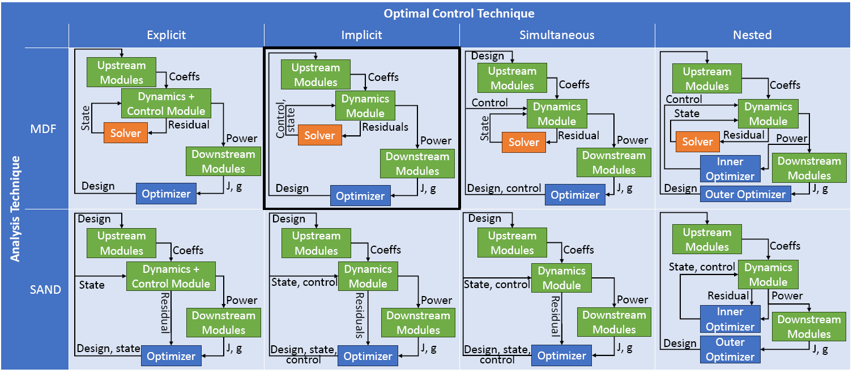
\includegraphics[width=\linewidth]{figs/img0009.png}
	
\end{frame}

\begin{frame}
	\frametitle{Dynamics: Nonlinearities with Describing Functions}
	
	\centering
	\begin{itemize}
		\item Approximate the non-sinusoidal signal with its fundamental amplitude
	\end{itemize}
	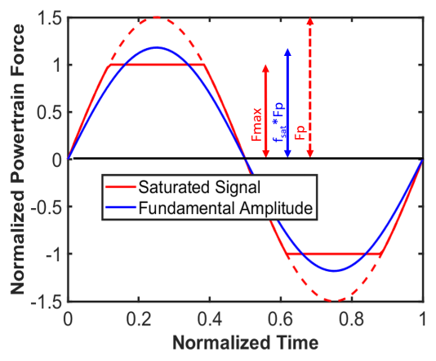
\includegraphics[width=0.6\linewidth]{figs/img0010.png}
	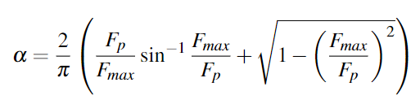
\includegraphics[width=0.4\linewidth]{figs/img0011.png}
	
	{\footnotesize McCabe, Murphy, and Haji, 2022.}
	
\end{frame}

\begin{frame}
	\frametitle{Dynamics: Linear Multiport Model}
	
	\centering
	\begin{itemize}
		\item Powertrain kinematics and dynamics
        \item Underactuated (fewer actuators than degrees of freedom)
	\end{itemize}
	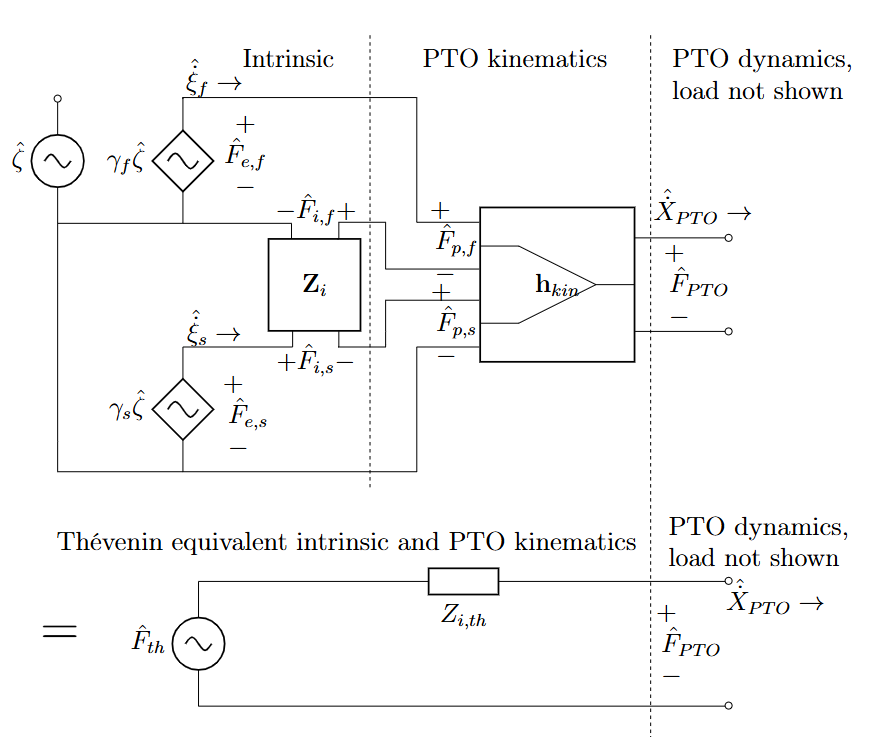
\includegraphics[width=0.7\linewidth]{figs/pto.png}
	
\end{frame}

\begin{frame}
	\frametitle{Controls: Linearized Pseudo-Spectral Method}
	
	\centering
	\begin{itemize}
		\item Incorporate time-domain constraints with collocation
        \item Apply describing function linearization
	\end{itemize}
	
\includegraphics[width=0.5\linewidth]{lin-ps-flow.png}
	%\includegraphics[width=0.4\linewidth]{example-image-a}
	
	{\footnotesize McCabe, Murphy, and Haji, 2022.}
	
\end{frame}

\begin{frame}
	\frametitle{Control: Quadratically Constrained Quadratic Program}
	
	\centering
	\begin{itemize}
		\item Convex in many cases
        \item Analytical solution for single actuated DOF in monochromatic waves
        \item Intersect circles in $\Gamma$ (reflection coefficient) space
	\end{itemize}
	\includegraphics[width=0.4\linewidth]{figs/qp_circles.pdf}
	%\includegraphics[width=0.4\linewidth]{example-image-a}
	
	{\footnotesize McCabe, Murphy, and Haji, 2022.}
	
\end{frame}

\begin{frame}
	\frametitle{Structural Analysis Methods}
	
	\centering
	\begin{itemize}
		\item Float: trapezoidal interpolation of rectangular plate solution
		\item Spar: short-column buckling
		\item Damping plate: annular plate bending with diagonal support
		\item All use equivalent-thickness method for stiffened plates
	\end{itemize}
	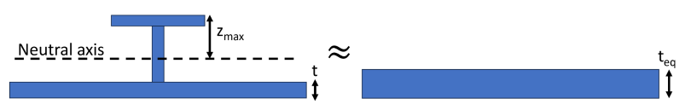
\includegraphics[width=0.9\linewidth]{figs/img0012.png}
	
	{\footnotesize McCabe, Dietrich, and Haji. “Development, Validation, and Benchmarking of a Multidisciplinary Semi-Analytical Model for Wave Energy Converters.” In preparation for submission to Applied Ocean Research.}
	
\end{frame}


\begin{frame}
	\frametitle{Synthesis: nondimensionalization and parameterization}
	
	\centering
	\begin{itemize}
		\item McCabe, Dietrich, Yang, Long, Kuan, Buccino, Liu, and Haji. “WEC optimization to maximize grid economic value and avoided emissions.” University Marine Energy Community Conference, August 2025, Corvallis OR.
	\end{itemize}
	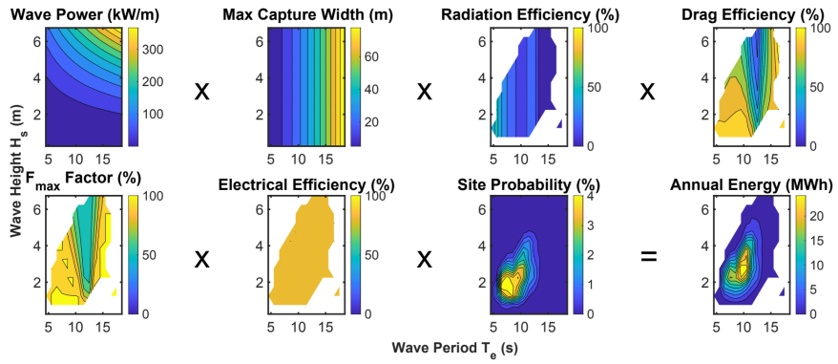
\includegraphics[width=0.9\linewidth]{figs/img0013.png}
	
\end{frame}


\begin{frame}
	\frametitle{Validation: error checking vs WEC-Sim ODE solver}
	
	\centering
	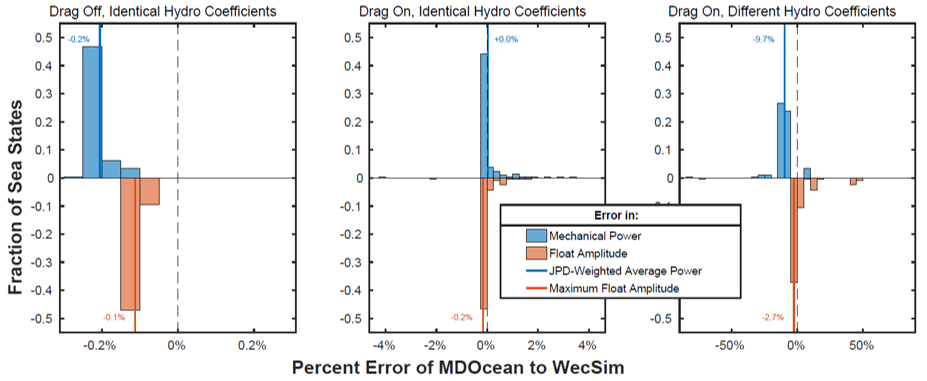
\includegraphics[width=0.9\linewidth]{figs/img0014.png}
	
	{\footnotesize McCabe, Dietrich, and Haji. “Development, Validation, and Benchmarking of a Multidisciplinary Semi-Analytical Model for Wave Energy Converters.” In preparation for submission to Applied Ocean Research.}
	
\end{frame}


\begin{frame}
	\frametitle{Benchmarking: time comparison vs standard numerical tools}
	
	\centering
	\begin{itemize}
		\item 100x faster hydro, 1000x faster dynamics
		      
		\item McCabe, Dietrich, and Haji. “Development, Validation, and Benchmarking of a Multidisciplinary Semi-Analytical Model for Wave Energy Converters.” In preparation for submission to Applied Ocean Research.
	\end{itemize}
    \begin{columns}
        \begin{column}{0.35\textwidth}
            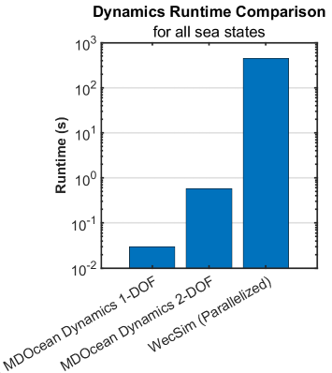
\includegraphics[0.35\textwidth]{figs/img0015.png}
        \end{column}
        
        \begin{column}{0.65\textwidth}
            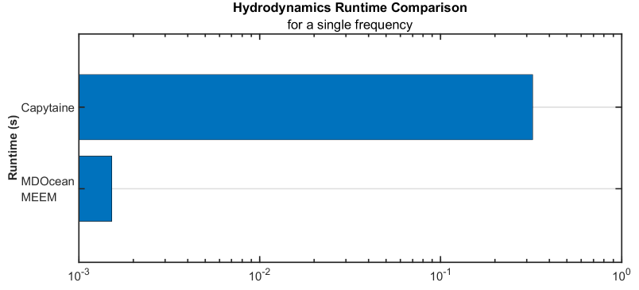
\includegraphics[0.65\textwidth]{figs/img0016.png}
        \end{column}
	   
    \end{columns}
	
	
\end{frame}
